\documentclass{book}
\usepackage[T1]{fontenc}
\usepackage[utf8]{inputenc}
\usepackage{lmodern}
\usepackage{microtype}
\usepackage{float}
\usepackage{blindtext}
\usepackage{physics}
\usepackage{breqn}
\usepackage{enumitem}
\setlist[itemize]{topsep=0pt, partopsep=0pt, parsep=0pt, itemsep=0pt}
\usepackage{setspace}
\setstretch{0.6515}

% Language
\usepackage[italian]{babel}

% Page Style
\pagestyle{myheadings}

% Layout and Geometry
\usepackage{layouts}
\usepackage[a2paper, top=0.5cm, bottom=0.5cm, left=0.5cm, right=0.5cm]{geometry}
\setlength\parindent{0pt}

% Section and Captions Formatting
\usepackage{titlesec}
\setcounter{secnumdepth}{5}
\setcounter{tocdepth}{5}
\usepackage{subcaption}
\captionsetup{justification=centering}
\usepackage{sidecap}

\titlespacing*{\section}
{0pt}{1ex}{0.5ex}
\titlespacing*{\subsection}
{0pt}{1ex}{0.4ex}

\setlength{\abovedisplayskip}{1pt}
\setlength{\belowdisplayskip}{1pt}
\setlength{\abovedisplayshortskip}{1pt}
\setlength{\belowdisplayshortskip}{1pt}

% Hyperlinks
\usepackage[breaklinks]{hyperref}
\hypersetup{
    colorlinks=true, 
    citecolor=blue,
    filecolor=red,
    linkcolor=dukeblue,
    urlcolor=blue
}
\def\UrlBreaks{\do\/\do-}

% Mathematics and Symbols
\usepackage{amsmath, amssymb, bm, siunitx, textcomp, gensymb}

% Graphics and Colors
\usepackage{graphicx, wrapfig}
\usepackage{xcolor}
%\usepackage{tikz}
%\usepackage{pgfplots}
%\pgfplotscolorbarCMYKworkaroundfalse

% Tables
\usepackage{array, multirow, longtable, booktabs, colortbl, adjustbox, hhline, diagbox, collcell}
\usepackage{tablefootnote, threeparttable, nicematrix}

% Lists and Formatting
\usepackage{enumitem}
\usepackage{dirtytalk}
\usepackage{comment}
\usepackage[splitrule]{footmisc}
\usepackage{multicol}
\usepackage{makecell}
\usepackage{changepage}

% Other Useful Packages
\usepackage{dblfloatfix}
\usepackage{lipsum}
\usepackage[absolute]{textpos}

% Code Listings
\usepackage{listings}

% Additions to Table of Contents
\addtocontents{toc}{\protect\thispagestyle{empty}}

% Commented Packages for Future Use
%\usepackage{breakurl}
%\usepackage{physics}
%\pgfplotsset{compat=1.3, width=7.5cm}
%\usetikzlibrary{pgfplots.fillbetween}
%\usepgfplotslibrary{external}
%\tikzexternalize
%\tikzexternalize[prefix=tikz/, optimize command away=\includepdf}
%\titlespacing*{\section}{0pt}{2pt}{2pt}
%\titlespacing*{\subsection}{0pt}{2pt}{2pt}
%\titlespacing*{\subsubsection}{0pt}{2pt}{2pt}
%\usepackage{anyfontsize}
%\usepackage{tabularray}



% comandi ---------------------------

\renewcommand{\arraystretch}{1.2}


\setlength{\arrayrulewidth}{0.41415mm}
\newcolumntype{s}{>{\columncolor{gray!20} m{2.5cm}}}
\def\changemargin#1#2{\list{}{\rightmargin#2\leftmargin#1}\item[]}
\let\endchangemargin=\endlist 
\newcommand\Item[1]{\item\begin{minipage}[t]{\linewidth}#1\end{minipage}}
\newcommand{\cov}{\mathrm{cov}}
\newcommand{\corr}{\mathrm{corr}}
\titleformat{\paragraph} 
{\normalfont\normalsize\bfseries} % Stile normale e grassetto
{\theparagraph} % Numerazione
{1em} 
{} 
\titlespacing\paragraph
{0pt} 
{3.25ex plus 1ex minus .2ex} 
{1.5ex plus .2ex} 


%------------------------------

% colori --------------------------------------

	\definecolor{almond}{rgb}{0.94, 0.87, 0.8}
\definecolor{dkgreen}{rgb}{0,0.6,0}
\definecolor{dukeblue}{rgb}{0.0, 0.0, 0.61}
\definecolor{mauve}{rgb}{0.58,0,0.82}
\definecolor{gold}{rgb}{1.0, 0.84, 0.0}
	\definecolor{amber}{rgb}{1.0, 0.749, 0.0}
\definecolor{jam}{rgb}{0.65, 0.04, 0.37}
\definecolor{darksalmon}{rgb}{0.91, 0.59, 0.48}
\definecolor{capello}{rgb}{0.8784,0.7373,0.6471}
	\definecolor{nastro}{rgb}{0.21, 0.27, 0.31}
 	\definecolor{azure}{rgb}{0.61, 0.87, 1.0}
\definecolor{hanblue}{rgb}{0.27, 0.42, 0.81}
 \definecolor{jade}{rgb}{0.0, 0.66, 0.42}
 \definecolor{jasper}{rgb}{0.84, 0.23, 0.24}
  	\definecolor{lav}{rgb}{0.8, 0.8, 1.0}
   \definecolor{emerald}{rgb}{0.31, 0.78, 0.47}
   	\definecolor{med}{rgb}{0.48, 0.41, 0.93}	
    \definecolor{ma}{rgb}{0.98, 0.93, 0.37}
    	\definecolor{silver}{rgb}{0.75, 0.75, 0.75}
     \definecolor{men}{rgb}{0.8, 0.8, 1.0}
     \definecolor{dartmouthgreen}{rgb}{0.05, 0.5, 0.06}
  	\definecolor{zaffre}{rgb}{0.0, 0.08, 0.66}
  	\definecolor{brass}{rgb}{0.71, 0.65, 0.26}
   \definecolor{green(html/cssgreen)}{rgb}{0.0, 0.5, 0.0}
   \definecolor{electricgreen}{rgb}{0.0, 1.0, 0.0}
   \definecolor{backcolour}{rgb}{0.95,0.95,0.92}
   \definecolor{forestgreen(web)}{rgb}{0.13, 0.55, 0.13}

%-------------------------

% Colori delle compatibilità ------------------
        \definecolor{ottima}{rgb}{0.47, 0.87, 0.47}
  	\definecolor{sufficiente}{rgb}{1.0, 0.7, 0.28}
       	\definecolor{incompatibile}{rgb}{1.0, 0.41, 0.38}
       \definecolor{buona}{rgb}{0.99, 0.99, 0.59}
% ----------------------------------------
% Colori accettato o meno ----------------
 \definecolor{accettato}{rgb}{0.47, 0.87, 0.47}
  \definecolor{rifiutato}{rgb}{1.0, 0.41, 0.38}
% programmi -----------------------

\lstdefinestyle{mystyle}{
frame=tb,
mathescape=true,
  aboveskip=3mm,
  belowskip=3mm,
  showstringspaces=false,
  columns=flexible,
  basicstyle=\ttfamily,
  numbers=left,
  backgroundcolor=\color{backcolour},   
  numberstyle=\color{zaffre},
  keywordstyle=\color{blue},
  commentstyle=\color{purple},
  stringstyle=\color{teal},
  breakatwhitespace=true,
  tabsize=3,
  breaklines=true
}
\lstset{style=mystyle, texcl=true}


\newcommand{\g}{\textbf}
\newcommand{\h}{\mathbf}
\newcommand{\e}{\begin{equation}} 
\newcommand{\ex}{\end{equation} }
\renewcommand{\it}{\item[$\cdot$]}

\begin{document}

\begin{multicols}{4}

\begin{itemize}
\item [$\blacksquare$] \g{MECCANICA AL FISSATO}
\item [$\blacktriangle$] \g{Operazioni in $L^2(\Delta)$}
    \it \g{Prodotto scalare}
        \e{\langle \varphi | \psi \rangle = \int_{\Delta} \varphi^*(x) \psi(x) \, dx = \overline{\langle \psi | \varphi \rangle}} \ex
    \it \g{Normalizzazione }
        \e{1 = \langle \psi | \psi \rangle = \int_{\Delta} \overline{\psi(x)}\psi(x) \, dx = \int_{\Delta} |\psi(x)|^2 \, dx = ||\psi||^{2}}     \ex
    \it \g{Autoaggiuntezza di un operatore}
        \e{\langle A\psi | \varphi \rangle = \langle \psi | A^\dagger \varphi \rangle = \langle \psi | A \varphi \rangle \quad A^{\dagger} = (A^{*})^{T} \quad (AB)^{\dagger} = B^{\dagger}A^{\dagger}} \ex
        
    \it \g{Norma di un operatore}
        \e{\|A\| = \sup_{\psi \in \mathcal{H} \setminus \{0\}} \frac{\|A\psi\|}{\|\psi\|} = \sup_{\|\psi\|=1} \|A\psi\|} \ex
    \it \g{Operatore che è funzione di un altro operatore}
        \e{f(A)\psi = f(a)\psi}\ex
        Vale se A è autoaggiunto e $\psi$ autofunzione
    \item [$\blacktriangle$] \g{Probabilità e statistica}
    \it \g{Probabilità di una misura}
    La probabilità che una misura dell'osservabile A nello stato $\left|\psi\right>$ sia $\text{a} \in \ \sigma_{d}(A) \  \text{è}  $ :
            \e{ {\text{P}_{\psi}(a)} = \sum_{r=1}^{d(a)}\frac{\left| \braket{a,r}{\psi} \right|^{2}}{\norm{\psi}^{2}}} \ex
       Mentre che sia $\in [a, \ a + \epsilon] \subseteq \sigma_{c}(A)$ è:    
\e{\int_{a}^{a+\epsilon}\rho_{\psi}\ \text{d}a \qquad  \text{dove} \qquad \rho_{\psi} = \sum_{r=1}^{d(a)}\frac{\left| \braket{a,r}{\psi} \right|^{2}}{\norm{\psi}^{2}}}\ex

\it \g{Probabilità di trovare la particella nell'intervallo $I \subseteq \Delta$}
        \e{\mathrm{Pr}(I) = \frac{\int_I |\psi(x)|^2\, dx}{||\psi||^{2}} \qquad \text{dove} \qquad ||\psi||^{2} =\int_{\Delta}|\psi|^{2}dx } \ex
Vale anche per qualsiasi altra rappresentazione di $\psi$ integrando nel corrispondente differenziale (ad esempio probabilità che la particella assuma un intervallo di momenti)

    \it \g{Teorema di Plancherel}
\e{\int_{\mathbb{R}}|\tilde{\psi}(p)|^{2}dp \   = \int_{\mathbb{R}}|\psi(x)|^{2}dx }\ex

        \it \g{Valor medio di un operatore nello stato $\left|\psi\right>$}
            \e{\langle A \rangle_{\psi}   =  \frac{\langle \psi | A | \psi \rangle}{||\psi||^{2}} = \sum_{a \ \in \ \sigma_{d}(A)}a \cdot \text{P}_{\psi}(a) + \int_{\sigma_{c}(A)} a \cdot \rho_{\psi}\ \text{d}a} \ex
        \it \g{Fluttuazione di un operatore}
        \e{(\Delta A)_{\hat{a}, \psi} = \sqrt{ \langle A^2 \rangle_\psi - \langle A \rangle_\psi^2}} \ex
        
    \item [$\blacktriangle$] \g{Operatore posizione X}
        \e{X\psi(x) = x\psi(x) \quad X^2\psi(x) = x^2\psi(x) \quad X^{-1}\psi(x) = \frac{1}{x} \psi(x)} \ex


\item [$\blacktriangle$] \g{Operatore momento P}
        \e{P = -i\hbar \frac{\partial}{\partial x} \quad P^2 = -\hbar^2 \frac{\partial^2}{\partial x^2}} \ex
    Se definito in un compatto $[0, L]$, le autofunzioni sono
        \e{\psi(x) = C \exp\left(\frac{i\lambda x}{\hbar}\right), \quad \lambda \in \mathbb{Z}} \ex
    ove si impone
        \e{\psi(0) = \psi(L)} \ex
    In particolare, se definito su una circonferenza, allora 
    \e {\lambda = \frac{n \hbar }{R}} \ex
    dove R è il raggio e $n \in \mathbb{Z}$
    \item[$\blacktriangle$] \g{equazione di Schrödinger in forma stazionaria}
        \e{\left[-\frac{\hbar^2}{2m} \nabla^2 + V\right] \psi(x) = E\psi(x)} \ex

 \item [$\blacktriangle$] \g{Dalla rappresentazione $\{x\}$ a $\{p\}$}
    Se si è in una dimensione
        \e{\tilde{\psi}(p) = \frac{1}{\sqrt{2\pi \hbar} }\int_{\mathbb{R}} e^{-\frac{ipx}{ \hbar}} \psi(x) \, dx \quad \psi(x) = \frac{1}{\sqrt{2\pi \hbar} }\int_{\mathbb{R}} e^{\frac{ipx}{\hbar}} \tilde{\psi}(p) \, dp} \ex
    Se si è in tre dimensioni invece tra $p$ e $x$ nell'exp va fatto il prodotto scalare, i differenziali sono in tre dimensioni e $\frac{1}{\sqrt{2 \pi \hbar}}$ diventa $\frac{1}{\left(2 \pi \hbar \right)^{3/2}}$
\item [$\blacktriangle$] \g{Indeterminazione di Heisenberg}
    \it \g{Espressione generale}
        \e{(\Delta A)_\psi (\Delta B)_\psi \geq \frac{1}{2}\left|{\langle [A, B] \rangle_\psi} \right|} \ex
        Valida se $\psi, A\psi, B\psi \ \in D_{A} \ \cap \ D_{B}$
        \it \g{Per la posizione e il momento}
        \e{(\Delta X)_{\psi}(\Delta P)_{\psi} \geq \frac{\hbar}{2}}\ex
        Che è sempre valida se se si lavora con $\mathcal{H} = L_{2}(\mathbb{R})$

\item [$\blacktriangle$] \g{Proiettori}
\e{\mathcal{P}^{+} = \mathcal{P} \qquad \mathcal{P}^{2} = \mathcal{P}}\ex
Gli autovalori di un proiettore sono 0 e 1 
\it \g{Utilizzo dei proiettori nel caso di spettro discreto}
Nel caso di $a \in \sigma_{d}(A)$ allora:
\e{\mathcal{P}_{a} = \sum_{r=1}^{d(a)}\ket{a,r}\bra{a,r}}\ex
\e{\sum_{a \ \in \ \sigma_{d}(A)}\mathcal{P}_{a} = \sum_{a \ \in \ \sigma_{d}(A)} \sum_{r = 1}^{d(a)}\ket{a,r}\bra{a,r} = \mathbb{I}}\ex

\e{\langle \mathcal{P}_{a} \rangle_{\psi} = \sum_{r=1}^{d(a)}\frac{|\braket{a,r}{\psi}|^{2}}{\norm{\psi}^{2}} = \frac{\norm{\mathcal{P}_{a}\ket{\psi}}^{2}}{\norm{\psi}^{2}} = \text{P}_{\psi}(a) \label{valor medio proiettore}}\ex

\it \g{Utilizzo dei proiettori nel caso di spettro generico }
\e{\mathcal{H} = \mathcal{H}_{s} \oplus \mathcal{H}_{s}^{\perp}}\ex
\e{S \subseteq \mathbb{R} }\ex
\e{\mathcal{P}_{s} = \sum_{a \ \in \ \sigma_{d}(A)\ \cap \ S} \sum_{r = 1}^{d(a)}\ket{a,r}\bra{a,r} + \int_{\sigma_{c}(A) \ \cap \ S} \sum_{r = 1}^{d(a)}\ket{a,r}\bra{a,r}\text{d}a   }\ex
$\langle \mathcal{P}_{s} \rangle_{\psi}$ è la  \text{Probabilità che una misura di A nello stato} $\psi$ \text{dia} $a \  \in \ S$
\item  [$\blacktriangle$] \g{Teoria della misura}
Lo stato prima della misura può essere descritto come 
\e{\ket{\psi} = \mathcal{P}_{a}\ket{\psi} + \left(\mathbb{I}-\mathcal{P}_{a}\right)\ket{\psi}}\ex
Dopo la misura lo stato diventa
\e{\ket{\psi} = \mathcal{P}_{a}\ket{\psi}}\ex
\it \g{Osservabili compatibili}
Siano A e B due operatori limitati e i relativi osservabili con spettro discreto. Allora valgono e  sono equivalenti le seguenti affermazioni:
\e{\mathcal{A} \ \text{e} \ \mathcal{B}\ \text{sono compatibili}}\ex
\e{ \exists \text{ una base o.n. } \{ \ket{a, b, r} \}_{\substack{a \in \sigma(A)  \\ b \in \sigma(B)  \\ r = 1, \dots, d(a, b)}}}\ex
Vale dunque $A\ket{a,b,r} = a\ket{a,b,r}$ e $B\ket{a,b,r} = b\ket{a,b,r}$
\e{[A,B] = 0}\ex
Inoltre valgono le seguenti due relazioni:
\e{[A,B] = 0 \implies [\mathcal{P}_{a}, \mathcal{P}_{b}] = 0 \ \forall a,b \iff [f(A), g(B)] = 0}\ex
\e{[A,B] = 0 \ \implies \ \forall b \ \in \sigma(B) \ \begin{cases}
   \  \forall \ket{b} \ \in \mathcal{H}_{b}, A\ket{b} \ \in \mathcal{H}_{b} \\
   [A, \mathcal{P}_{b}] = 0
    \label{commutatore A e Pb}
    
\end{cases}}\ex
\it \g{ICOC}
Si tratta di un insieme completo di osservabili compatibili, si può indicare con $\vec{A}$. 
\e{\vec{A} \ \text{ICOC} \iff d(\vec{a}) = 1 \ \forall \vec{a} \ \in \ \sigma_{\vec{A}}}\ex
La base o.n. di un ICOC sarà $\{\ket{\vec{a}}\}_{\vec{a} \ \in \ \sigma(\vec{A})}$
\item [$\blacktriangle$] \g{Quantizzazione canonica}
\e{\{ \, \} = \frac{1}{i \hbar} \left[ \, , \, \right]}\ex
\item [$\blacksquare$] \g{Evoluzione temporale causale}
\item [$\blacktriangle$] \g{Equazione di Schrödinger in forma temporale}
        \e{i\hbar \frac{\partial}{\partial t} \psi(t) = H\psi(t)} \ex
    Dove $i \hbar \frac{\partial}{\partial t} $ è l'espressione dell'operatore Energia.
Una combinazione lineare di soluzioni è ancora una soluzione. Per ogni dato iniziale $\ket{\psi(0)}$ si avrà un'unica soluzione $\forall t$. Infine $\norm{\psi(t)}$ si conserva nel tempo. 
Inoltre $\psi^{*}$ è soluzione dell'equazione
\e{-i \hbar \frac{\partial}{\partial t} \psi^{*}(t) = H\psi^{*}(t) }\ex
\item [$\blacktriangle$] \g{Equazione di continuità}
\e{\frac{d}{dt}{\rho(\vec{x},t)} + \vec{\nabla} \cdot \vec{J}(\vec{x},t) = 0}\ex
dove 
\e{\rho(\vec{x},t) = |\psi(\vec{x},t)|^{2}}\ex è la densità di probabilità, mentre
\e{\vec{J}(\vec{x},t) = -\frac{i\hbar}{2m}\left(\psi^{*}\vec{\nabla} \psi  - \psi \vec{\nabla} \psi^{*}\right) }\ex
è la densità di corrente di probabilità.\\
In una dimensione e senza dipendenza temporale essa diventa:
\e{\frac{d}{dx}\left(\psi'\psi^{*} - (\psi^{*})'\psi\right) = 0}\ex
\item [$\blacktriangle$] \g{Operatore di evoluzione causale}
\e{U^{-1}(t,t_{0}) = U^{+}(t,t_{0}) = U(t_{0},t)}\ex
In un sistema conservativo, in cui cioè l'hamiltoniana resta invariata nel tempo, si ha 
        \e{U(t) = \exp\left(-i\frac{t}{\hbar}H\right)} \ex

    \item [$\blacktriangle$] \g{Visuale di Schroedinger}
        \e{|\psi(t)\rangle = U(t) |\psi(t_{0})\rangle} \ex
        Sia $\ket{E_{n}, r}$ l’autoket dell’autovalore $E_n$, allora, per quanto riguarda la parte di spettro discreto
        \e{|\psi(t)\rangle = \sum_n \sum_{r=1}^{d(E_{n})}\exp\left(-\frac{i}{\hbar} E_n(t - t_0)\right) \braket{E_{n}, r}{\psi(t_{0})} \ket{E_{n},r}} \ex
        Se poi c'è anche una parte continua di spettro si aggiunge
        \e{\int_{\sigma_{c}(H)}d\text{E}\sum_{r=1}^{d(E)}\exp\left(-\frac{i}{\hbar} E(t - t_0)\right) \braket{E, r}{\psi(t_{0})} \ket{E,r}}\ex
        \it \g{Stati stazionari}
Un autostato dell'hamiltoniana, $\ket{\psi_{E}}$ viene chiamato stato stazionario ed evolve in questo modo:
\e{\ket{\psi_{E}(t)} = \text{exp}\left(-\frac{i}{h}E(t-t_{0})\right)\ket{\psi_{E}(t_{0})}}\ex
il valor medio e la varianza di un operatore calcolati su uno stato stazionario non variano nel tempo:
\e{\frac{d}{dt}\langle A \rangle_{\psi_{E}} = 0, \qquad \frac{d}{dt}(\Delta A)^{2}_{\psi_{E}} = 0 \quad \forall A} \label{valor medio stato stazionario}\ex
\it \g{Operatori}       
In visuale di Schroedinger gli operatori rimangono invariati:
\e{A \rightarrow \ A}\ex
\item [$\blacktriangle$] \g{Visuale di Heisenberg}
    \it \g{Equazione di Born-Heisenberg-Jordan}
        \e{\frac{d}{dt} X_h(t) = \frac{[X_h(t), H]}{i\hbar} + \left(\frac{\partial A}{\partial t}\right)_{h}(t)} \ex
        dove l'ultimo termine è presente solo se A dipende esplicitamente dal tempo
    \it \g{Trasformazione unitaria}
        In visuale di Heisenberg, la trasformazione unitaria $U(t, t_{0})$ trasforma l’operatore $A_{s}$ (operatore A in visuale di Schroedinger) come:
        \e{A \to A_{h} = U^\dagger(t, t_{0}) A_{s} U(t, t_{0})} \ex
        mentre gli stati rimangono invariati:
        \e{\psi \to \psi} \ex
        In particolare $\ket{\psi}$ in visuale di Heisenberg sarà uguale al ket in visuale di Schroedinger all'istante iniziale:
        \e{\ket{\psi_{h}(t)} = \ket{\psi_{h}(t_{0})} = \ket{\psi_{s}(t_{0})}}\ex
        \it \g{Valori medi di operatori}
        In visuale di Heisenberg e di Schroedinger i valori medi degli operatori coincidono:
        \e{\langle A_{s}\rangle = \langle A_{h}\rangle}\ex
        Inoltre
        \e{\frac{d}{dt}\langle A_{h}\rangle_{\psi}(t) = \frac{\langle \psi_{h} | \frac{d}{dt}A_{h}| \psi_{h}\rangle}{\norm{\psi_{h}}^{2}}}\ex
        \e{\frac{d}{dt}A_{h} = 0 \  \implies \frac{d}{dt}\langle A_{h}\rangle = 0}\ex
        \item [$\blacktriangle$] \g{Teorema di Ehrenfest}
        \e{\frac{d}{dt}\langle Q \rangle_{\psi} = \frac{\langle P \rangle_{\psi}}{m} \qquad \frac{d}{dt}\langle P \rangle_{\psi} = - \langle V'(Q) \rangle_{\psi}}\ex
        \item [$\blacktriangle$] \g{Indeterminazione tempo energia}
        \e{(\Delta t)_{\psi}(\Delta E)_{\psi} \gtrsim \frac{\hbar}{2}}\ex
        \item [$\blacktriangle$] \g{Operatori densità}
        Per uno stato puro si ha 
        \e{\rho_{\psi} = \frac{\ket{\psi}\bra{\psi}}{\norm{\psi}^{2}}}\ex
        \e{\rho_{nm} = \langle n|\rho|m\rangle = \braket{n}{\psi}\braket{\psi}{m} = C_{n}C_{m}^{*}}\ex
        $\rho$, per uno stato puro, è un proiettore per cui valgono le proprietà dei proiettori. Inoltre per uno stato puro valgono 
        \e{\sigma(\rho) \geq 0 \qquad Tr(\rho^{2}) = 1} \ex
        Dove Tr è la traccia
        \e{\langle A \rangle_{\psi} = \text{Tr}(\rho A)}\ex
        Per uno stato misto $\epsilon$ si ha 
        \e{\rho_{\epsilon} = \sum_{k}P_{k}\ket{\psi_{k}}\bra{\psi_{k}}}\ex
        Dove le $P_{k}$ sono le probabilità associate agli stati puri $\psi_{k}$, per cui la loro somma deve essere uguale a 1.
        Inoltre si ha 
        \e{\langle A \rangle_{\epsilon} = \sum_{k}P_{k}\langle A_{k}\rangle = Tr(\rho_{\epsilon}A)}\ex
        Infine per uno stato misto si ha 
        \e{Tr(\rho^{2}) < 1} \ex
        Per quanto riguarda l'evoluzione casuale si ha:
        \e{\rho_{s}(t) = \sum_{k}P_{k}\ket{\psi_{k}(t)}\bra{\psi_{k}(t)} = U(t,t_{0})\rho(t_{0})U(t,t_{0})^{\dagger}}\ex
        \e{\langle A \rangle(t) = Tr(U \rho(t_{0})U^{\dagger}A) = Tr(\rho(t_{0})U^{\dagger}AU) = Tr(\rho(t_{0})A_{h})} \ex
        \e{i \hbar \frac{d}{dt}\rho_{s}(t) = [H_{s}(t), \rho_{s}(t)]}\ex
        
     
\item [$\blacksquare$] \g{Simmetrie}
\it \g{Teorema di Wigner}
\e{\tau \ \text{è una trasformazione di simmetria} \iff \begin{cases}
    \psi^{'} = W \psi\\
    A' = WAW^{\dagger}
\end{cases}}\ex 
Con U operatore unitario o antiunitario

\item [$\blacktriangle$] \g{Traslazioni spaziali}
    \it \g{Operatore di traslazione}
        \e{U(\varphi) = \exp\left(-i\frac{\varphi}{\hbar} P\right)} \ex
        dove $\varphi$ è il parametro di traslazione e P è il generatore infinitesimo di traslazione
        \it \g{Effetto sull'operatore di posizione e sul momento}
        \e{X' = U(\varphi)XU(\varphi)^{\dagger} = X -\varphi \qquad U(\varphi)^{\dagger}XU(\varphi) = X +\varphi}\ex
        \e{U(\varphi) P = P} \ex
    \it \g{Effetto sulla funzione d'onda}
        \e{U(\varphi)\psi(x) = \psi(x - \varphi)} \ex
    \it \g{Traslazioni in 3D}
    Le relazioni sono analoghe a quelle in 1D, semplicemente vanno espresse vettorialmente. Inoltre
    
     \e{U(\vec{\varphi}) = \text{exp}\left(-\frac{i}{\hbar}\vec{P}\cdot \vec{\varphi}\right)}\ex
\item [$\blacktriangle$] \g{Rotazioni}
    \it \g{Operatore di rotazione}
        \e{U(\vec{\varphi}) = \exp\left(-i\frac{\vec{\varphi} \cdot \vec{J}}{\hbar}\right)} \ex
        $\vec{J}$ è dunque il generatore infinitesimo di rotazione
        
    \it \g{Matrice di rotazione attorno all'asse z}
        \e{R(\varphi, \hat{z}) = 
        \begin{pmatrix}
            \cos\varphi & -\sin\varphi & 0\\ 
            \sin\varphi & \cos\varphi & 0 \\
            0 & 0 & 1
        \end{pmatrix}} \ex
    \it \g{Effetto sulle coordinate e momento}
        \e{X' = U^\dagger X U = R^{-1}(\vec{\varphi}) X \qquad P' = U^\dagger P U = R^{-1}(\vec{\varphi}) P} \ex

    \item[$\blacktriangle$] \g{Simmetrie della dinamica}
Sono quelle simmetrie tali per cui
\e{[W,H] = 0 \ \iff \ WHW^{\dagger} = H \ \iff \ [W, U(t-t_{0})] = 0}\ex
dove $U(t-t_{0})$ in questo caso è l'operatore di evoluzione causale. Da questa relazione si ricava banalmente la validità della seguente relazione:
\e{\langle H \rangle_{\psi({t})} = 0 \quad \forall \ket{\psi(t)}}\ex se H non dipende dal tempo
\it \g{Gruppo a un parametro di simmetrie della dinamica}
Definito 
\e{W(\varphi) = \text{exp}\left(-\frac{i}{\hbar}Q\varphi\right)}\ex con $W(s) \in G_{d}$ (gruppo di simmetrie della dinamica) e Q generatore infinitesimo della simmetria, si ha 
\begin{align}
    [W(s), H] &= 0 \iff [Q, H] = 0 
    &\iff \frac{d}{dt} \langle Q \rangle_{\psi}(t) = 0 \quad \forall \psi \in \mathcal{H}
\end{align}
E ciò se e solo se Q è una costante del moto. Si noti inoltre che non si conserva solo il valor medio di Q ma anche tutte le probabilità associate agli autovalori di Q, per via della (\ref{commutatore A e Pb}) e della (\ref{valor medio proiettore}).
\it \g{Esempio con Hamiltoniana in una dimensione}
Ad esempio per un oscillatore armonico in direzione x, come nel caso della (\ref{oscillatore armonico}), siccome $P_{y}$ e $P_{z}$ commutano con H, i loro valori medi non varieranno nel tempo. Il valor medio di $P_{x}$ invece non varierà nel tempo, in generale, solo se calcolato su uno stato stazionario di H (si veda la (\ref{valor medio stato stazionario})).

\it \g{Simmetrie della dinamica e autostati dell'energia}

W mescola autostati di H con la stessa energia, per cui essa è una matrice a blocchi. Si ha 
\e{[W, H] = 0 \ \iff \ \forall \ket{E} \ \in \mathcal{H}_{E},\  W \ket{E} \ \in \ \mathcal{H}_{E}}\ex
dove $\mathcal{H}_{E}$ è l'autospazio dell'hamiltoniano relativo all'autovalore E, e inoltre $H\ket{E} = E\ket{E}$

    
\item [$\blacktriangle$] \g{Operatore parità}
    \it \g{azione dell’operatore parità sulla funzione d'onda}
        \e{P\psi(x) = \psi(-x)} \ex
    \it \g{Spettro e autofunzioni}
        Lo spettro è
        \e{\sigma(P) = \{\pm 1\}} \ex
        e la degenerazione degli autovalori è infinita. 
        \e{\begin{cases}
          P\psi(x) = \psi(x) \quad   \text{se} \ \psi(x) \ \text{è pari}\\
          P\psi(x) = -\psi(x) \quad \text{se dispari}
        \end{cases}}\ex

    \it \g{Trasformato per parità}
        Il trasformato per parità di un generico operatore $A$ è
        \e{PAP^\dagger} \ex
        Nel caso dell’oscillatore armonico, per gli operatori di distruzione e creazione:
        \e{PaP^\dagger = -a \qquad
        Pa^\dagger P^\dagger = -a^\dagger} \ex
        E per gli operatori posizione e momento:
        \e{P\vec{X}P^\dagger = -\vec{X} \qquad P\vec{P}P^\dagger = -\vec{P} \qquad P\vec{L}P^{\dagger} = \vec{L}} \ex
\it \g{Attenzione alla parità}
    La parità su una funzione traslata agisce solo sulla variabile indipendente e non sul fattore di traslazione. Ovvero:
        \e{Pf(x - 2a) = f(-x - 2a)} \ex
    Se invece si effettua la trasformazione:
        \e{f(x - 2a) \to f(-x + 2a)} \ex
    Si è effettuata una riflessione intorno all’asse $x = a$.
    \it \g{Parità come simmetria della dinamica}
    l'Operatore parità rappresenta una simmetria della dinamica quando commuta con H. Ad esempio se per l'hamiltoniana 
    \e{H = \frac{\vec{P}^{2}}{2m} + V(\vec{X})}\ex 
    si ha $V(\vec{X}) = V(-\vec{X})$, come nel caso dell'oscillatore armonico, allora le autofunzioni dell'hamiltoniana hanno parità definita. Esse sono anche autofunzioni della parità in quanto H e la parità saranno operatori compatibili. Ciò significa inoltre che considerato un generico stato, se questo ad esempio è pari, si può decomporre in autostati pari dell'hamiltoniana.
\item [$\blacktriangle$] \g{Inversione temporale}
Essa manda t in -t
\it \g{Azione sugli operatori}
\e{\mathcal{T}\vec{X} \mathcal{T}^{\dagger} = \vec{X} \qquad \mathcal{T} \vec{P} \mathcal{T}^{\dagger} = - \vec{P}}\ex
\it \g{Azione sulla funzione d'onda}
\e{\mathcal{T}\psi(x) = \psi^{*}(x)}\ex
\it \g{Inversione temporale e evoluzione causale}
\e{\mathcal{T}U(t)\mathcal{T}^{\dagger} = U(-t)}\ex 
dove $U(t)$ è l'operatore di evoluzione causale.
\e{\mathcal{T}\ket{\psi(-t)} = U(t)\mathcal{T}\ket{\psi(0)} \qquad \mathcal{T}\psi(\vec{x},t) = \psi^{*}(\vec{x},-t)}\ex
    
  
\item [$\blacktriangle$] \g{Commutazioni generiche e altre formule}
    \it \g{Commutatori di base}
        \e{[X_i, P_j] = i\hbar\delta_{ij} \qquad [\vec{X}, \vec{P}] = i \hbar\  \mathbb{I} \qquad [Q,f(P)] = i \hbar f'(P)}\ex
        \e{[A,B] = 0 \ \implies [f(A),B] = 0 \qquad [A,f(A)] = 0}\ex
        dove Q è l'operatore di posizione generalizzata
        \e{[X, P^2] = 2i\hbar P \qquad [X^2, P^2] = 4i\hbar XP + 2\hbar^2} \ex
    \it \g{Commutatori con l'operatore di traslazione}
    \e{[Q, U(\varphi)] = \varphi \ U(\varphi)}\ex
    \it \g{Formula di Baker-Campbell-Hausdorff}
    \e{e^{A}e^{B} = e^{A + B + \frac{1}{2}[A, B] + \frac{1}{12}\left([A,[A,B]] + [B,[B,A]]\right)\ + \dots} }\ex
    
\item[$\blacksquare$] \g{Formule utili da Fisica moderna}
\item [$\blacktriangle$] \g{Particella libera }
 \e{-\frac{\hbar^2}{2m} \frac{d^2}{dx^2} \varphi_E(x) = E \varphi_E(x) \Rightarrow 
            \frac{d^2}{dx^2} \varphi_E(x) + k^2 \varphi_E(x) = 0} \ex
            \e{k = \sqrt{\frac{2mE}{\hbar^{2}}}
            }\ex
            La soluzione è
            \e{\psi_{s}(x,t) = C_{+}e^{i(kx - \omega t)} + C_{-}e^{-i(kx - \omega t)}}\ex
            dove il primo termine è un'onda che va verso dx mentre il secondo è un'onda che va verso sx.
    \it \g{Dominio dell’hamiltoniana di una particella libera}
        \e{D(H) = \left\{ \psi(x) \in L^2(\mathbb{R}, dx), \, p^2 \tilde{\psi}(p) \in L^2(\mathbb{R}, dp) \right\}} \ex
    Quando il potenziale è $C^\infty$ ed è limitato in tutto $\mathbb{R}$ allora il dominio dell’hamiltoniana del sistema è lo stesso di quella libera.
\item [$\blacktriangle$] \g{Energia e momento quantizzati}
Per un quanto di energia si ha
\e{E = \hbar \omega \qquad P = \hbar k = \hbar \frac{2 \pi}{\lambda} = \frac{ \hbar \omega}{c}}\ex
\item [$\blacktriangle$] \g{Buca infinita}
    \it \g{Buca di potenziale infinitamente profonda, posta in $[-L/2, +L/2]$}
        \it \g{Equazione agli autovalori}
            \e{-\frac{\hbar^2}{2m} \frac{d^2}{dx^2} \varphi_E(x) = E \varphi_E(x) \Rightarrow 
            \frac{d^2}{dx^2} \varphi_E(x) + k^2 \varphi_E(x) = 0} \ex
        \it \g{Soluzioni}
            \e{\varphi_n(x) = 
            \begin{cases} 
                \sqrt{\frac{2}{L}} \cos\left(\frac{n\pi x}{L}\right), & n > 0 \text{ dispari} \\
                \sqrt{\frac{2}{a}} \sin\left(\frac{n\pi x}{L}\right), & n > 0 \text{ pari}
            \end{cases}} \ex
        \it \g{Autovalori di $H$}
            \e{E_n = \frac{\hbar^2}{2m} \left(\frac{n\pi}{L}\right)^2} \ex
    \it \g{Buca di potenziale infinitamente profonda, posta in [0,L]}
    L'energia rimane la stessa, mentre le autofunzioni sono
    \e{\varphi_{n} = \sqrt{\frac{2}{L}}\sin(\frac{n \pi x}{L}) \ \forall \ n > 0}\ex
    
    
\item [$\blacktriangle$] \g{Gradino di potenziale}
    Potenziale a gradino $V(x) = \bar{V} \Theta(x)$, con $\Theta(x)$ funzione di Heaviside.

    \it \g{Autofunzioni}
    Si pone
    \e{\chi = \sqrt{\frac{2m(\bar{V} - E)}{\hbar^2}} \qquad k = \sqrt{\frac{2mE}{\hbar^2}}} \ex

    \it \g{Con energia minore di $\bar{V}$}
    \e{\varphi_E(x) = 
    \begin{cases}
        c_+^1 e^{ikx} + c_-^1 e^{-ikx}, & x < 0 \\
        c_2^- e^{-\chi x}, & x \geq 0
    \end{cases}} \ex

    \it \g{Con energia maggiore di $\bar{V}$}
    \e{\varphi_E(x) = 
    \begin{cases}
        c_+^1 e^{ikx} + c_-^1 e^{-ikx}, & x < 0 \\
        c_2^+ e^{\chi x}, & x \geq 0
    \end{cases}} \ex

   \item [$\blacksquare$] \g{Oscillatore armonico}
    \it \g{Pulsazione}
        \e{\omega = \sqrt{\frac{k}{m}}} \ex

    \it \g{Hamiltoniana}
        \e{H = \frac{P^2}{2m} + \frac{1}{2}m\omega^2 X^2 + V_0 = \hbar\omega\left(a^\dagger a + \frac{1}{2}\right) + V_0} \label{oscillatore armonico}\ex

    \it \g{Spettro di $H$}
        \e{ E_{n} = \hbar\omega\left(n + \frac{1}{2}\right) + V_0, \quad n \in \mathbb{N}\ \text{U} \ \{0\}\ } \ex
    \it \g{Commutazione con la parità}
        \e{[P, H] = 0} \ex

    \it \g{Autofunzioni}
        \e{\psi_0(x) = \left(\frac{m\omega}{\pi\hbar}\right)^{1/4} \exp\left(-\frac{m\omega}{2\hbar}x^2\right)} \ex
        \e{\psi_1(x) = \left(\frac{m\omega}{\pi\hbar}\right)^{1/4} \sqrt{\frac{2m\omega}{\hbar}} x \exp\left(-\frac{m\omega}{2\hbar}x^2\right)} \ex
        \e{\psi_2(x) = \frac{1}{\sqrt{8}} \left(\frac{m\omega}{\pi\hbar}\right)^{1/4} \exp\left(-\frac{m\omega}{2\hbar}x^2\right)\left(4\frac{m\omega}{\hbar}x^2 - 2\right)} \ex
        \e{\psi_n(x) = \frac{1}{\sqrt{2^n n!}} \left(\frac{m\omega}{\pi\hbar}\right)^{1/4} \exp\left(-\frac{m\omega x^2}{2\hbar}\right) H_n\left(\sqrt{\frac{m\omega}{\hbar}} x\right)} \ex
        Dove $H_n(y)$ sono i polinomi di Hermite:
        \e{H_n(y) = (-1)^n e^{y^2} \frac{d^n}{dy^n} e^{-y^2}} \ex
        \e{H_0(y) = 1, \quad H_1(y) = 2y, \quad H_2(y) = 4y^2 - 2} \ex
        \it \g{Proprietà delle autofunzioni}
        Ortogonalità:
        \e{\langle m | n \rangle = \delta_{mn}} \ex
        \e{\int_{\mathbb{R}} \psi_i(ax) \psi_j(ax) = \frac{\delta_{ij}}{a}} \ex
     Le autofunzioni sono a parità definita, ovvero sono pari per indici pari, dispari per indici dispari:
     \e{\psi_{n}(-x) = (-1)^{n}\psi_{n}(x)}\ex
     \e{\langle X \rangle_{\psi_{n}} = \langle P \rangle_{\psi_{n}} = 0 \qquad \langle 
     X^{2}\rangle_{\psi_{n}} = \frac{\hbar}{m \omega}(n + \frac{1}{2})}\ex
     In generale il valor medio di $X$ su domini simmetrici e su stati $\ket{\psi}$ a parità definita è nullo.
     \e{\langle P^{2}\rangle_{\psi_{n}} = \hbar \omega m (n + \frac{1}{2}) \ \implies \langle \frac{P^{2}}{2m}\rangle_{\psi_{n}} = \frac{E_{n}}{2}}\ex
     Ovvero l'energia è equamente divisa, in media, tra parte cineticia e parte potenziale. 

     \it \g{Teorema di Ehrenfest per l'oscillatore armonico}
     Le soluzioni delle due equazioni differenziali per l'oscillatore armonico sono 
     \e{\langle X \rangle_{\psi} = A\cos(\omega t + \delta) \quad \left\langle P \right\rangle_{\psi} = - m A \omega \sin(\omega t + \delta)}\ex
     \it \g{Evoluzione temporale oscillatore armonico}
    $\ket{\psi(t)}$ nel caso dell'oscillatore armonico è periodica con periodo 
    \e{T = \frac{2 \pi}{\omega}}\ex
    
\item [$\blacktriangle$] \g{Operatori di creazione e distruzione}
    \it \g{Operatori definiti}
        \e{X' = \sqrt{\frac{m\omega}{\hbar}} X, \quad P' = \frac{1}{\sqrt{m\hbar\omega}} P} \ex
        \e{a = \frac{X' + iP'}{\sqrt{2}}, \quad a^\dagger = \frac{X' - iP'}{\sqrt{2}}} \ex

    \it \g{Relazioni di commutazione}
        \e{[a, a^\dagger] = 1} \ex

    \it \g{Espressioni per $X$ e $P$}
        \e{X = \sqrt{\frac{\hbar}{2m\omega}} (a + a^\dagger) \qquad P = i{\sqrt{\frac{m \hbar \omega}{2}}} (a^\dagger - a)} \ex

    \it \g{Azioni degli operatori}
        \e{a^\dagger |n\rangle = \sqrt{n + 1} |n + 1\rangle \qquad a |n\rangle = \sqrt{n} |n - 1\rangle} \ex
        \e{(a^\dagger)^2 |n\rangle = \sqrt{(n + 1)(n + 2)} |n + 2\rangle }\ex
        \e{a^2 |n\rangle = \sqrt{n(n - 1)} |n - 2\rangle} \ex
        \e{a a^\dagger |n\rangle = (n + 1) |n\rangle, \quad a^\dagger a |n\rangle = n |n\rangle} \ex
        \e{P |n\rangle = (-1)^n |n\rangle = (-1)^N |n\rangle} \ex
        \e{\psi_n(x) = \frac{(a^\dagger)^n}{\sqrt{n!}} \psi_0(x) \qquad \ket{n} = \frac{(a^{\dagger})^{n}}{\sqrt{n!}}\ket{0}} \ex
\item [$\blacktriangle$] \g{Operatore numero}
        \e{N = a^\dagger a \qquad N\ket{n} = n\ket{n} \qquad N a \ket{n} = (n-1)a\ket{n}}\ex
    \it \g{Relazioni di commutazione}
        \e{[N, a] = -a, \quad [N, a^\dagger] = a^\dagger} \ex
    
\item [$\blacksquare$] \g{Momento angolare}
\item [$\blacktriangle$] \g{Momento angolare totale}
        Il momento angolare totale è
        \e{\vec{J} = \vec{L} + \vec{S}}\ex
            dove $\vec{L}$ è il momento angolare orbitale, mentre $\vec{S}$ è lo spin
        \e{{J}^{2} = J^{2}_{x} + J^{2}_{y} + J^{2}_{z}}\ex
        Formule analoghe per $L^{2}$ e $S^{2}$
         \it \g{Autovalori di $J^2$ e $J_z$}
    \e{J^2 |l, m\rangle = \hbar^2 j(j + 1) |j, m\rangle \qquad L_z |j, m\rangle = \hbar m |j, m\rangle} \ex
      con $j \in \frac{1}{2} \mathbb{N}$ e $m \in \{-j, -j + 1, \dots, +j\}$.
    \item [$\blacktriangle$] \g{Momento angolare orbitale}
        \e{\vec{L} = \vec{X} \cross \vec{P} \qquad L_k = \sum_{i,j}\epsilon_{kij} X_i P_j} \ex
    \e{L_{x} = YP_{z} - ZP_{y} \quad L_{y} = ZP_{x} - XP_{z} \quad L_{z} = XP_{y} - YP_{x}}\ex
    \it \g{Autovalori di $L^2$ e $L_z$}
    \e{L^2 |l, m\rangle = \hbar^2 l(l + 1) |l, m\rangle \qquad L_z |l, m\rangle = \hbar m |l, m\rangle} \ex

    \it \g{Espressioni di $L^2$, $L_{x}$, $L_{y}$ e $L_{z}$}
    \e{L^2 = -\hbar^2 \left[ \frac{\partial^{2}}{\partial \theta^{2}} + \frac{1}{\tan(\theta)}\frac{\partial}{\partial  \theta} + \frac{1}{\sin^2\theta} \frac{\partial^2}{\partial \varphi^2} \right]} \ex
    \e{L_{x} = i \hbar \left[\sin(\varphi) \frac{\partial}{\partial \theta} + \cos(\varphi)\cot(\theta)\frac{\partial}{\partial \varphi}\right]}\ex
    \e{ L_{y} = i \hbar\left[-\cos(\varphi)\frac{\partial}{\partial \theta} + \sin(\varphi)\cot(\theta)\frac{\partial}{\partial\varphi}\right]}\ex
\e{L_{z} = - i \hbar \frac{\partial}{\partial \varphi}}\ex
    \item [$\blacktriangle$] \g{Operatori di abbassamento e innalzamento}
        \e{L_\pm = \hbar e^{\pm i\varphi} \left[i\cot\theta \frac{\partial}{\partial\varphi} \pm \frac{\partial}{\partial\theta}\right]} \ex
        \e{J_\pm = J_x \pm iJ_y, \quad J_- = (J_+)^\dagger} \ex
        \e{J_\pm |j, m\rangle = \hbar \sqrt{j(j+1) - m(m \pm 1)} |j, m \pm 1\rangle \label{azione J+ J-}} \ex
        Nella base $\ket{j,m}$, con m che va in ordine da j a $-j$, $J_{z}$ risulta diagonalizzata, $J_{+}$ ha valori non nulli solo nella diagonale sopra quella principale, $J_{-}$ ha valori non nulli solo nella diagonale sotto quella principale. Per costruire $L_{\pm}$, $L_{x}$ e $L_{y}$ le formule sono analoghe a queste ma con l al posto di j.
         \e{J_z J_\pm |j, m\rangle = \hbar(m \pm 1) J_\pm |j, m\rangle} \ex
         \e{J_{+}J_{-} = J^{2} - J_{z}\left(J_{z} - \hbar\right) \qquad J_{-}J_{+} = J^{2} - J_{z}\left(J_{z} + \hbar\right)}\ex
Valgono formule analoghe per $L_{+}$, $L_{-}$ e $S_{+}$, $S_{-}$
    \it \g{Espressione di $J_x$ e $J_y$}
        \e{J_x = \frac{J_+ + J_-}{2} \qquad J_y = \frac{J_+ - J_-}{2i} \label{Jx e Jy}} \ex

        

    \item [$\blacktriangle$] \g{Relazioni di commutazione}
    \begin{equation}
\varepsilon_{ijk} =
\begin{cases}
+1 & \text{se } (i,j,k) \text{ è una permutazione pari di } (1,2,3) \\
-1 & \text{se } (i,j,k) \text{ è una permutazione dispari di } (1,2,3) \\
\ \ 0 & \text{se due indici sono uguali}
\end{cases}
\end{equation}
        \e{[J_{i},L_{j}] = [L_i, L_j] = i\hbar \epsilon_{ijk} L_k \quad [L^2, L_j] = 0 \quad[J_i, J_j] = i\hbar \epsilon_{ijk} J_k } \ex \e{[L_i, X_j] = [J_i, X_j] = i\hbar \epsilon_{ijk} X_k \quad [L_i, P_j] = [J_i, P_j] = i\hbar \epsilon_{ijk} P_k} \ex
         \e{[J_z, J_\pm] = \pm \hbar J_\pm \qquad [J_+, J_-] = 2\hbar J_z} \ex
       

\item [$\blacktriangle$] \g{Autofunzioni simultanee di $L^{2}$ e $L_{z}$}
La forma generica è data da 
\e{\psi_{l}^{m} = f_{l}^{m}(r)Y_{l}^{m}(r,\theta,\varphi) \label{autofunzioni simultanee L2 e Lz}}\ex
dove 
    \e{Y^m_l(\theta, \varphi) = \frac{(-1)^{l}}{2^{l}l!}\sqrt{\frac{(2l + 1)}{4\pi} \frac{(l + m)!}{(l - m)!}}e^{im\varphi} P^m_l(\cos(\theta), \sin(\theta)) } \ex
    vengono dette armoniche sferiche. $P^m_l(\cos(\theta), \sin(\theta))$ è un polinomio in $\cos(\theta)$ e $\sin(\theta)$. In termini di polinomi di Legendre, si ha:
    \e{P^m_l(x) = (-1)^m \frac{(1 - x^2)^{m/2}}{2^l l!} \frac{d^{l+m}}{dx^{l+m}} (x^2 - 1)^l} \ex
    Le armoniche sferiche sono ortonormali:
    \e{\int_{0}^{2\pi}\text{d}\varphi\int_{0}^{\pi}\text{d}\theta \sin(\theta)\overline{Y_{l}^{m}(\theta,\varphi)}Y_{l'}^{m'}(\theta,\varphi) = \delta_{ll'}\delta_{mm'}}\ex
    dove $\int_{0}^{2\pi}\text{d}\varphi\int_{0}^{\pi}\text{d}\theta \sin(\theta) = \int\text{d}\Omega$\\
    Inoltre valgono le seguenti proprietà:
    \e{Y_{l}^{m}(\pi - \theta,\varphi + \pi) = (-1)^{l}Y_{l}^{m}(\theta,\varphi)}\ex
    \e{\overline{Y_{l}^{m}(\theta,\varphi)} = (-1)^{m}Y_{l}^{-m}(\theta,\varphi)}\ex
    Per la funzione radiale bisogna imporre la normalizzazione seguente:
    \e{\int_{0}^{+\infty} r^{2} |f_{l}^{m}(r)|^{2}\text{d}r = 1}\ex
\it \g{Armoniche sferiche: Primi valori}
    Le armoniche sferiche sono pari se $l$ è pari, dispari altrimenti.

    \it \g{Per $l = 0$}
        \e{Y^0_0(\theta, \varphi) = \frac{1}{\sqrt{4\pi}}} \ex

    \it \g{Per $l = 1$}
        \e{Y^0_1(\theta, \varphi) = \sqrt{\frac{3}{4\pi}} \cos\theta = \sqrt{\frac{3}{4\pi}} \frac{z}{r}} \ex
        \e{Y^{\pm 1}_1(\theta, \varphi) = \mp \sqrt{\frac{3}{8\pi}} \sin\theta e^{\pm i\varphi} = \mp \sqrt{\frac{3}{8\pi}} \frac{x \pm iy}{r}} \ex

    \it \g{Per $l = 2$}
        \e{Y^0_2(\theta, \varphi) = \frac{1}{4} \sqrt{\frac{5}{\pi}} (3\cos^2\theta - 1) = \frac{1}{4} \sqrt{\frac{5}{\pi}} \frac{(2z^2 - x^2 - y^2)}{r^2}} \ex
        \e{Y^{\pm 1}_2(\theta, \varphi) = \mp\frac{1}{2} \sqrt{\frac{15}{2\pi}} e^{\pm i\varphi} \sin\theta \cos\theta = -\frac{1}{2} \sqrt{\frac{15}{2\pi}} \frac{z(x \pm iy)}{r^2}} \ex
        \e{Y^{\pm 2}_2(\theta, \varphi) = \frac{1}{4} \sqrt{\frac{15}{2\pi}} e^{\pm 2i\varphi} \sin^2\theta = \frac{1}{4} \sqrt{\frac{15}{2\pi}} \frac{(x \pm iy)^2}{r^2}} \ex
        \item [$\blacksquare$] \g{Prodotto tensore}
        \e{\lambda \ket{\psi_{1}} \otimes \ket{\psi_{2}} = \lambda (\ket{\psi_{1}} + \ket{\psi_{2}}) \ \forall \lambda \ \in\  \mathbb{C}}\ex
\e{\ket{\psi_{1}} \otimes (\ket{\chi_{2}} + \ket{\psi_{2}}) = \ket{\psi_{1}} \otimes \ket{\chi_{2}} + \ket{\psi_{1}} \otimes \ket{\psi_{2}}}\ex
\e{\left\{ \ket{e_{1,n}} \otimes \ket{e_{2,m}} \right\}_{\substack{n = 1,\dots,d_1 \\ m = 1,\dots,d_2}}}\ex
è una base o.n. di $\mathcal{H} = \mathcal{H}_{1} \otimes \mathcal{H}_{2}$, dove
\e{\text{dim}(\mathcal{H}_{1} \otimes \mathcal{H}_{2}) = (\text{dim}\mathcal{H}_{1})(\text{dim}\mathcal{H}_{2})}\ex
    \item [$\blacktriangle$]\g{Prodotto scalare}
\begin{align}
    \braket{\psi}{\psi'} &= \left(\sum_{n,m}c_{n,m}^{*
}\bra{e_{1,n}}\otimes\bra{e_{2,m}}\right)\left(\sum_{n',m'}d_{n',m'}\ket{e_{1,n'}}\otimes\ket{e_{2,m'}}\right) \\
&= \sum_{n,n',m,m'}c_{n.m}^{*}d_{n',m'}\delta_{n,n'}\delta_{m.m'} = \sum_{n,m}c_{n.m}^{*}d_{n,m}
\end{align}
Tra due vettori fattorizzati si ha 
\e{(\bra{\psi_{1}}\otimes \bra{\psi_{2}})(\ket{\chi_{1}}\otimes\ket{\chi_{2}}) = \braket{\psi_{1}}{\chi_{1}}_{\mathcal{H}_{1}}\braket{\psi_{2}}{\chi_{2}}_{\mathcal{H}_{2}}}\ex
     \item [$\blacktriangle$]\g{Norma}
\e{\norm{\psi}^{2} = \sum_{n,m}|c_{n,m}|^{2}}\ex
\item [$\blacktriangle$] \g{Operatori e prodotto tensore}
\e{(A_{1} \otimes B_{2})\left(\sum_{n,m}C_{n,m}\ket{e_{1,n}} \otimes \ket{e_{2,m}}\right) = }\ex
\e{ = \sum_{n,m}C_{n,m}\left(A_{1}\ket{e_{1,n}}\right) \otimes \left(B_{2}\ket{e_{2,m}}\right)}\ex
\e{(A_{1} \otimes \mathbb{I}_{\mathcal{H}_{2}})(\mathbb{I}_{\mathcal{H}_{1}} \otimes B_{2}) = A_{1} \otimes B_{2} = (\mathbb{I}_{\mathcal{H}_{1}} \otimes B_{2})(A_{1} \otimes \mathbb{I}_{\mathcal{H}_{2}})}\ex
\e{A_{1}\ \text{a.a e }\{\ket{a_{1,r}}\}_{\substack{a_{1} \ \in \sigma(A_{1})\\ r = 1, \dots, d(a1)}} \text{base o.n. di } \mathcal{H}_{1} \label{base A1}}\ex
\e{B_{2} \ \text{a.a e }\{\ket{b_{2,s}}\}_{\substack{b2 \ \in \sigma(B2)\\ s = 1, \dots, d(b2)} } \text{base o.n. di } \mathcal{H}_{2} \label{base B2}}\ex
\e{(\ref{base A1}) \ \text{e} \ (\ref{base B2}) \implies \{\ket{a_{1,r}} \otimes \ket{b_{2,s}}\}_{\substack{a1 \ \in \sigma(A1), r = 1, \dots,d(a1) \\ b2 \ \in \ \sigma(B2), s = 1, \dots,d(b2)}}} \ex
è base o.n. di $\mathcal{H} = \mathcal{H}_{1} \otimes \mathcal{H}_{2}$. Dati due autovalori $a_{1}$ e $b_{2}$ fissati, la degenerazione della coppia su $\mathcal{H}$ sarà
\e{d(a_{1},b_{2}) = d(a_{1})d(b_{2})}\ex
\item [$\blacksquare$] \g{Spin}
\it \g{Hamiltoniana di interazione con $\vec{B}$}
\e{H = -\vec{\mu}\cdot \vec{B} \qquad \vec{\mu} = \mu_{0}\vec{S}}\ex
    \it \g{Relazioni di commutazione}
        \e{[S_i, S_j] = i\hbar \epsilon_{ijk} S_k \qquad [S_{i},X_{j}] = [S_{i}, P_{j}] = [S_{i}, L_{j}] = 0} \ex
        \e{[L^{2}, S^{2}] = 0 \qquad [J^{2}, S^{2}] = 0 \qquad [J^{2}, L^{2}] = 0 \qquad [S^{2}, S_{z}] = 0}\ex
    \it \g{Spettro di $(S^2, S_z)$}
        \e{\sigma(S^2; S_z) = \{\hbar^2 s(s+1), \hbar m\}} \ex
        con $s \in \frac{1}{2} \mathbb{N}$ e $m \in \{-s, -s + 1, \dots, +s\}$.
\item [$\blacktriangle$] \g{Prodotto $L \cdot S$}
    \e{L \cdot S = \frac{1}{2} \left(J^2 - L^2 - S^2\right)} \ex
    \e{L \cdot S = L_{z}S_{z} + \frac{1}{2}(L_{+}S_{-} + L_{-}S_{+})}\ex
\item [$\blacktriangle$] \g{Spin $1/2$}
         \it\g{Operatori di abbassamento e innalzamento}
         Per $S{\pm}$ vale l'analogo della (\ref{azione J+ J-}) con s al posto di j, per $S_{x}$ e $S_{y}$ vale l'analogo della (\ref{Jx e Jy}) cutilizzando $S_{\pm}$
  \it\g{Matrici di Pauli}
    \e{S = \frac{\hbar}{2} \sigma} \ex
    \e{\sigma_x = 
    \begin{pmatrix}
        0 & 1 \\
        1 & 0
    \end{pmatrix} \quad \sigma_y = 
    \begin{pmatrix}
        0 & -i \\
        i & 0
    \end{pmatrix} \quad \sigma_z = 
    \begin{pmatrix}
        1 & 0 \\
        0 & -1
    \end{pmatrix}} \ex
    \e{\sigma_{z}\ket{+} = \ket{+} \qquad \sigma_{z}\ket{-} = - \ket{-}}\ex
    \e{[\sigma_i, \sigma_j] = 2i \epsilon_{ijk} \sigma_k \qquad \{\sigma_i, \sigma_j\} = 2\delta_{ij}} \ex
    \e{\sigma_i \sigma_j = \frac{1}{2} \left([\sigma_i, \sigma_j] + \{\sigma_i, \sigma_j\}\right)} \ex
\it \g{Composizione di spin di due particelle}
    \e{S^{(1)} \cdot S^{(2)} = \frac{1}{2}\left(S^{(1)}_+ S^{(2)}_- + S^{(1)}_- S^{(2)}_+\right) + S^{(1)}_z S^{(2)}_z} \ex
\it \g{Spin in direzione $\hat{n}$}        
    Sia $\hat{n}$ il versore in $\mathbb{R}^3$:
    \e{\hat{n} = (\sin\theta\cos\varphi, \sin\theta\sin\varphi, \cos\theta)} \ex
    \e{S \cdot \hat{n} = \frac{\hbar}{2} \sigma \cdot \hat{n} = \frac{\hbar}{2}
    \begin{pmatrix}
        \cos\theta & \sin\theta e^{-i\varphi} \\
        \sin\theta e^{i\varphi} & -\cos\theta
    \end{pmatrix}} \ex
       \e{\sigma(S_n) = \left\{-\frac{\hbar}{2}, +\frac{\hbar}{2}\right\}} \ex

    Gli autostati sono:
    \e{|+\rangle_{\hat{n}} = \cos\frac{\theta}{2}  |+\rangle + \sin\frac{\theta}{2} e^{i{\varphi}} |-\rangle} \ex
    \e{|-\rangle_{\hat{n}} = \sin\frac{\theta}{2} |+\rangle - \cos\frac{\theta}{2} e^{i{\varphi}} |-\rangle} \ex
in forma matriciale gli autostati lungo una generica direzione $\hat{n}$ sono:
    \e{\left|\frac{\hbar}{2}\right\rangle_{\hat{n}} =
    \begin{pmatrix}
        \cos\frac{\theta}{2}  \\
        \sin\frac{\theta}{2} e^{i{\varphi}}
    \end{pmatrix} \qquad \left|-\frac{\hbar}{2}\right\rangle_{\hat{n}} =
    \begin{pmatrix}
        \sin\frac{\theta}{2}  \\
        -\cos\frac{\theta}{2} e^{i{\varphi}}
    \end{pmatrix}} \ex
\it \g{Spin in direzione $x$}
    \e{|+\rangle_x = \frac{1}{\sqrt{2}}(|+\rangle + |-\rangle) \qquad |-\rangle_x = \frac{1}{\sqrt{2}}(|+\rangle - |-\rangle)} \ex
    \e{|+\rangle = \frac{1}{\sqrt{2}}(|+\rangle_x - |-\rangle_x) \qquad |-\rangle = \frac{1}{\sqrt{2}}(|+\rangle_x + |-\rangle_x)} \ex
\it \g{Spin in direzione $y$}
    \e{|+\rangle_y = \frac{1}{\sqrt{2}}(\ket{+} + i\ket{-}) \quad |-\rangle_y = \frac{1}{\sqrt{2}}(|+\rangle -i|-\rangle)} \ex
    \e{|+\rangle = \frac{1}{\sqrt{2}}(|+\rangle_y + |-\rangle_y) \quad |-\rangle = -\frac{i}{\sqrt{2}}(|+\rangle_y - |-\rangle_y)} \ex
    \it \g{Spinore di Pauli}
    Considerando gli spazi di posizione e di spin assieme, ovvero $\mathcal{H} = \mathcal{H}_{\vec{x}} \ \otimes \ \mathcal{H}_{\vec{s}} $ lo stato della particella di spin 1/2 è descritto dallo spinore di Pauli:
    \e{\ket{\psi} = \begin{pmatrix}
        \psi_{+}(\vec{x})\\
        \psi_{-}(\vec{x} 
    \end{pmatrix} = [\psi](\vec{x}) = \psi_{+}(\vec{x})\begin{pmatrix}
        1 \\ 0
    \end{pmatrix} + \psi_{-}(\vec{x}) \begin{pmatrix}
        0 \\ 1
    \end{pmatrix}}\ex
    \e{\psi_{+}(\vec{x}) = \braket{\vec{x}, +}{\psi} \quad \psi_{-}(\vec{x}) = \braket{\vec{x},-}{\psi}}\ex
    \e{\norm{\psi}^{2} = \int \text{d}x^{3}\left(\left|\psi_{+}(\vec{x})\right|^{2} + \left|\psi_{-}(\vec{x})\right|^{2}\right)}\ex
    \e{(\vec{X}\left[\psi\right])(\vec{x}) = \begin{pmatrix}
        \vec{x}\psi_{+}(\vec{x})\\
        \vec{x}\psi_{-}(\vec{x})
    \end{pmatrix} \quad (\vec{P}[\psi])(\vec{x}) = -i \hbar \begin{pmatrix}
        \vec{\nabla}\psi_{+}(\vec{x})\\
        \vec{\nabla}\psi_{-}(\vec{x})
    \end{pmatrix} }\ex
    \e{(\vec{S}[\psi])(\vec{x}) = \frac{\hbar}{2}\vec{\sigma}\begin{pmatrix}
        \psi_{+}(\vec{x})\\
        \psi_{-}(\vec{x})
    \end{pmatrix}}\ex
\item [$\blacksquare$] \g{Composizione dei momenti angolari}
    \it \g{Generalità}
        \e{J = J^{(1)} \otimes I + I \otimes J^{(2)}} \ex
        dove ad esempio per una particella con spin $J^{(1)} = L$ e $J^{(2)} = S$, mentre per due particelle senza spin $J^{(1)} = L^{(1)}$ e $J^{(2)} = L^{(2)}$. Possiamo diagonalizzare simultaneamente $\{J^{2 \ (1)}, J^{(1)}_z,J^{2 \ (2)}, J^{(2)}_z\}$ oppure $\{J^{2 \ (1)}, J^{2 \ (2)}, J^{2},J_{z}\}$ per cui si può scrivere
        \e{\ket{j1,j2,j,m} \equiv \ket{j,m} = \sum_{m1,m2}\ket{m1,m2}\braket{m1,m2}{j,m}}\ex
        dove $\braket{m1,m2}{j,m}$ vengono detti coefficienti di Clebsch Gordan. Si noti inoltre, che siccome essi possono essere scelti reali, si ha anche 
        \e{\ket{j1,j2,m1,m2} \equiv \ket{m1,m2} = \sum_{j,m} \ket{j,m}\braket{m1,m2}{j,m}}\ex 
         \e{j \ \in \{j_{1} + j_{2}, j_{1} + j_{2} - 1, \dots, |j_{1}-j_{2}|\}}\ex
        \e{J_{z}\ket{j,m} = \hbar m\ket{j,m} \qquad J_{z}\ket{m1,m2} = (m1 + m2)\hbar \ket{m1,m2}}\ex
    \it \g{Relazioni di commutazione}
        \e{[J^2, J^{(1)}] = 0 \qquad [J^2, J^{(2)}] = 0 \qquad [J^2, J^{(1,2)}_i] \neq 0} \ex
        \it \g{Coefficienti di Clebsch-Gordan} Ogni coefficiente, ad esempio $-3/2$, va letto come se ci fosse una radice. In questo caso quindi $-\sqrt{3/2}$. I numeri in alto, ad esempio $1 \cross 1$, indicano nell'ordine i valori di $j_{1}$ e $j_{2}$
         \begin{minipage}[t]{1.1\linewidth}
        \centering
        \begin{minipage}[t]{0.3\linewidth} % Prima immagine
            \centering
            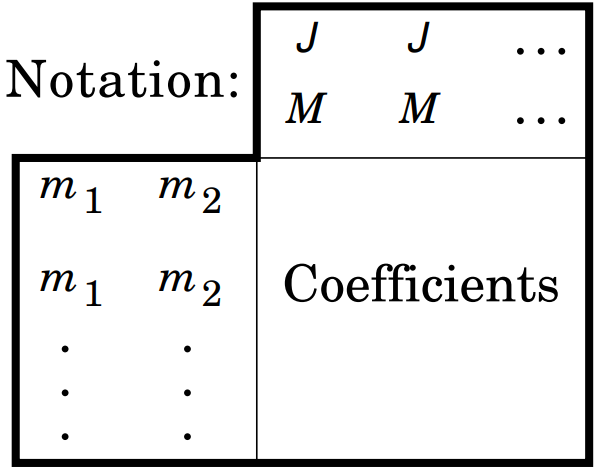
\includegraphics[width=\linewidth]{Immagini/notation.png}
        \end{minipage}%
        \hfill
        \begin{minipage}[t]{0.7\linewidth} % Seconda immagine
            \centering
            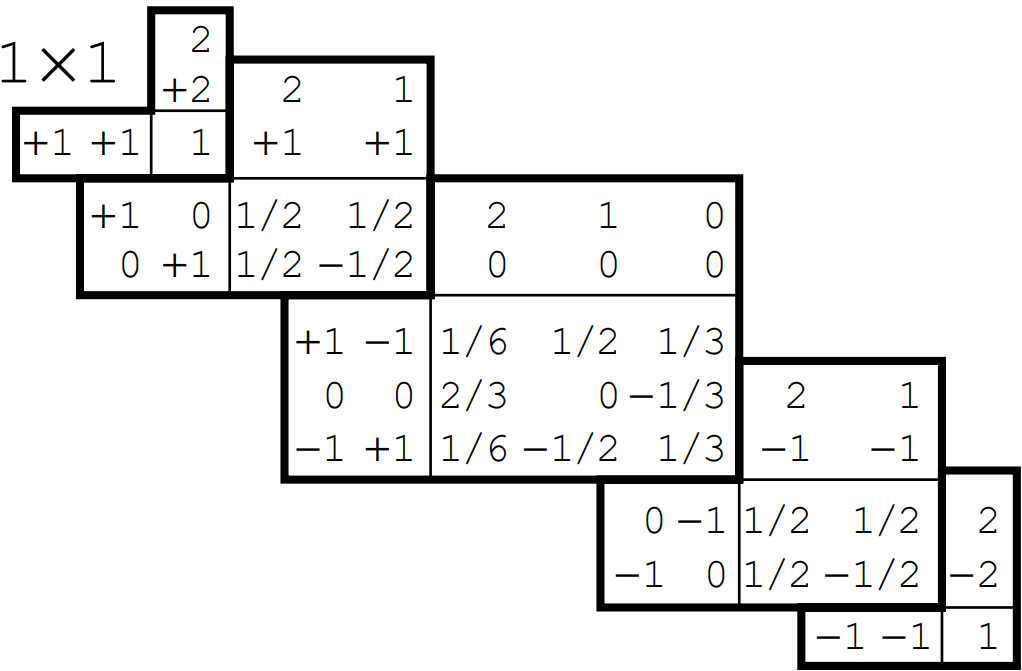
\includegraphics[width=\linewidth]{Immagini/11.png}
        \end{minipage}
    \end{minipage}
 
    \begin{minipage}[t]{1.05\linewidth}
        \centering
        \begin{minipage}[t]{0.42\linewidth} % Prima immagine
            \centering
            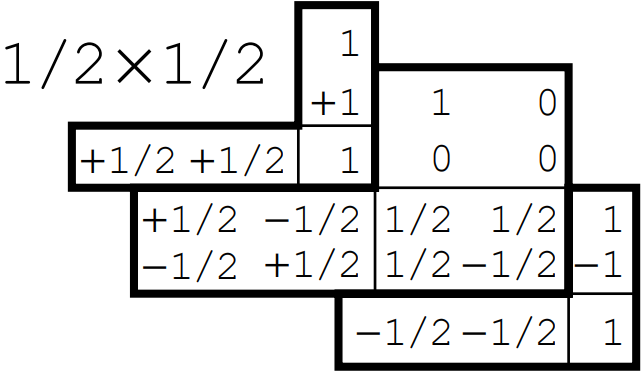
\includegraphics[width=\linewidth]{Immagini/1212.png}
        \end{minipage}%
        \begin{minipage}[t]{0.62\linewidth} % Seconda immagine
            \centering
            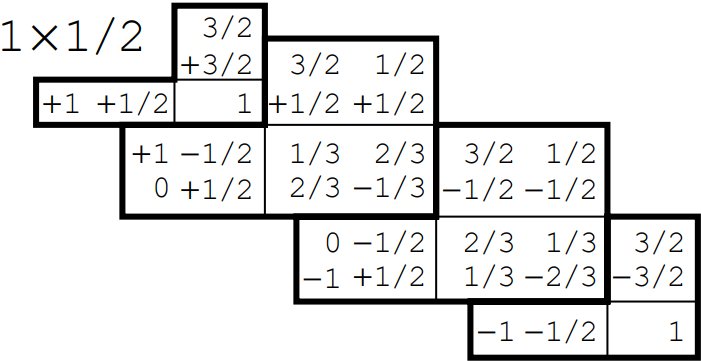
\includegraphics[width=\linewidth]{Immagini/112.png}
        \end{minipage}
    \end{minipage}
    
\item [$\blacksquare$] \g{Particelle identiche }
I bosoni hanno spin intero, ovvero $s \ \in \mathbb{Z}$ mentre i fermioni semi intero, ovvero $s \ \in \frac{1}{2} + \mathbb{Z}$.
Sotto lo scambio di etichette la funzione d'onda complessiva dei bosoni deve essere simmetrica, quella dei fermioni antisimmetrica (ovvero deve acquistare un segno - nel caso di due particelle). 

\item [$\blacktriangle$] \g{Due particelle identiche di spin $\frac{1}{2}$}
Considerato lo spazio di Hilbert
\e{\mathcal{H}^{\otimes 2} = \mathcal{H}_{\vec{X_{1}}, \vec{X_{2}}} \otimes \mathcal{H}_{\vec{S_{1}}, 
\vec{S_{2}} }}\ex

Si possono diagonalizzare simultaneamente 
$ \{ \vec{X}_1, \vec{X}_2, S_{1,z}, S_{2,z} \}$ oppure $ \{ \vec{X}_1, \vec{X}_2, S^{2}, S_{z} \}$. Espandendo quest'ultima base data da $\{\ket{s,m}\}$ nella base della prima, data da $\{\ket{m1, m2}\}$, tramite i coefficienti di Clebsch-Gordan, si ottiene:
\e{\ket{1,1} = \ket{+,+} \quad \ket{1,0} = \frac{1}{\sqrt{2}}\left(\ket{+-} + \ket{-+}\right) \quad \ket{1,-1} = \ket{--}}\ex
che vengono detti stati di tripletto e sono simmetrici
\e{\ket{s=0,m=0} = \frac{1}{\sqrt{2}}\left(\ket{+-} - \ket{-+}\right)}\ex
che viene detto stato di singoletto ed è asimmetrico. 
Per quanto detto sopra allora le parti di posizione per tali particelle dovranno essere antisimmetriche nel caso degli stati di tripletto e simmetriche nel caso del singoletto. 

\item [$\blacksquare$] \g{Atomo di Idrogeno}
$\{ H, L^{2},L_{z}\}$ è un ICOC
\item [$\blacktriangle$] \g{Hamiltoniana separata in due parti}
\e{H = H_{CM} + H_{r} \quad M = m_{a} + m_{b}}\ex
\e{\vec{X}_{CM} = \frac{m_{a}}{M}\vec{X_{a}} + \frac{m_{b}}{M}\vec{X_{b}} \quad \vec{P}_{CM} = \vec{P_{a}} + \vec{P_{b}}}\ex
\e{\vec{X_{r}} = \vec{X_{a}} - \vec{X_{b}} \quad \vec{P_{r}} = \frac{m_{b}}{M}\vec{P_{a}} - \frac{\vec{m_{a}}}{M}\vec{P_{b}}}\ex
\e{H_{r} = \frac{\vec{P}^{2}_{r}}{2 \mu} - \frac{e^{2}}{r} \qquad \mu = \frac{m_{e}m_{p}}{M}}\ex
\item [$\blacktriangle$] \g{Autofunzioni e autovalori per stati legati}
Le autofunzioni sono del tipo della (\ref{autofunzioni simultanee L2 e Lz}). Gli autovalori $E_{n}$, con n=1 stato fondamentale, hanno degenerazione $n^{2}$. In particolare per ogni livello n si hanno autofunzioni per tutti i valori di l e m che rispettano tali condizioni:
\e{0 \leq l  \leq n-1 \qquad -l \leq m \leq l}\ex
Gli autovalori hanno energia pari a 
\e{E_{n} = - \frac{E_{I}}{n^{2}}}\ex
\item [$\blacksquare$] \g{Teoria delle perturbazioni}
    \it \g{Hamiltoniana perturbata}
        \e{H = H_0 + \lambda V = H_0 + W} \ex
    \it \g{Equazioni agli autovalori}
        \e{H_0 |E_n^0\rangle = E_n^0 |E_n^0\rangle, \quad H |E_n\rangle = E_n |E_n\rangle} \ex
\item [$\blacktriangle$] \g{Risoluzione nei casi senza degenerazione}
\e{E_{n}^{\lambda} = E_{n}^{0} + \lambda E_{n}^{1} + \lambda^{2}E_{n}^{2} + \dots}\ex
\e{\ket{E_{n}^{\lambda}} = \ket{E_{n}^{0}} + \lambda \ket{E_{n}^{1}} + \lambda^{2}\ket{E_{n}^{2}} + \dots}\ex
    \it \g{Primo e secondo ordine}
        \e{E_n^1 = \langle E_n^0 | V | E_n^0 \rangle \qquad E_n^{2} = \sum_{m \neq n} \frac{|\langle E_n^0 | V | E_m^0 \rangle|^2}{E_n^0 - E_m^0}} \ex
        \e{\ket{E_{n}^{1}} =  \sum_{m \neq n} \ket{E_{m}^{0}}\frac{\langle E_m^0 | V | E_n^0 \rangle}{E_n^0 - E_m^0}}\ex
    \item [$\blacktriangle$] \g{Risoluzione nei casi con degenerazione}
    Si costruisce la matrice $V$ con dimensione pari al valore della degenerazione. Per trovarne gli elementi si usa 
    \e{\braket{\psi_{r}|V}{\psi_{s}}}\ex dove $\ket{\psi_{r}}$ e $\ket{\psi_{s}}$ sono autovettori degeneri relativi allo stesso autovalore. Diagonalizzando V si trovano le correzioni $E_{n,1}^{k}$ relative agli sviluppi
    \e{E^{k} = E_{n, 0}^{k} + \lambda E_{n,1}^{k} + \dots}\ex
    Gli autovettori della matrice V sono invece gli autovettori all'ordine 0 espressi nella base degli autovettori degeneri.
    \item [$\blacksquare$] \g{Dimensioni fisiche}
    \e{[\ \hbar\ ] = [\ E\ ][\ T\ ] \qquad [\ \omega \  ] = [\ T \ ]^{-1} }\ex
    \e{ \text{In 3D} \ [\ |\psi| \ ] = [\ L\ ]^{-3/2}, \quad \text{In 1D} \ [\ |\psi| \ ] = [\ L\ ]^{-1/2} }\ex
    \e{ \text{In 2D} \ [\ |\psi| \ ] = [\ L\ ]^{-1}}\ex
    \e{\left[ \ \vec{E} \ \right] = \frac{[\ E \ ]}{[ \ L \ ][ \ Q \ ]} \qquad \left[ \ \vec{B} \ \right] = \frac{[\ E \ ][\ T \ ]}{[\ Q \ ][\ L \ ]^{2}}}\ex
    
\item [$\blacksquare$] \g{Matematica utile}
    \item [$\blacktriangle$] \g{Identità trigonometriche}
        \e{\cos\alpha = \frac{e^{i\alpha} + e^{-i\alpha}}{2}, \quad \sin\alpha = \frac{e^{i\alpha} - e^{-i\alpha}}{2i}} \ex
        \e{\cosh(\alpha) = \frac{e^{\alpha} + e^{-\alpha}}{2}\qquad \sinh(\alpha) = \frac{e^{\alpha} - e^{-\alpha}}{2} }\ex

    \it \g{Formule di duplicazione}
        \e{\sin(2\alpha) = 2\sin\alpha\cos\alpha \quad \tan(2\alpha) = \frac{2\tan\alpha}{1 - \tan^2\alpha}} \ex
        \e{\cos(2\alpha) = \cos^2\alpha - \sin^2\alpha = 1 - 2\sin^2\alpha = 2\cos^2\alpha - 1} \ex
        \e{\sin^2\alpha = \frac{1 - \cos(2\alpha)}{2}, \quad \cos^2\alpha = \frac{1 + \cos(2\alpha)}{2}} \ex

    \it \g{Formule di bisezione}
        \e{\cos\frac{\alpha}{2} = \pm\sqrt{\frac{1 + \cos\alpha}{2}}, \quad \sin\frac{\alpha}{2} = \pm\sqrt{\frac{1 - \cos\alpha}{2}}} \ex
        \e{\tan\frac{\alpha}{2} = \pm\sqrt{\frac{1 - \cos\alpha}{1 + \cos\alpha}} = \frac{1-\cos\alpha}{\sin\alpha}=\frac{\sin\alpha}{1+\cos\alpha}} \ex

    \it \g{Formule parametriche}
        Sia $t = \tan\frac{\alpha}{2}$ con $\alpha \neq (2k + 1)\pi$, allora:
        \e{\sin\alpha = \frac{2t}{1 + t^2}, \quad \cos\alpha = \frac{1 - t^2}{1 + t^2}} \ex

    \it \g{Formule di prostaferesi}
        \e{\sin\alpha + \sin\beta = 2\sin\left(\frac{\alpha + \beta}{2}\right)\cos\left(\frac{\alpha - \beta}{2}\right)} \ex
        \e{\sin\alpha - \sin\beta = 2\cos\left(\frac{\alpha + \beta}{2}\right)\sin\left(\frac{\alpha - \beta}{2}\right)} \ex
        \e{\cos\alpha + \cos\beta = 2\cos\left(\frac{\alpha - \beta}{2}\right)\cos\left(\frac{\alpha + \beta}{2}\right)} \ex
        \e{\cos\alpha - \cos\beta = -2\sin\left(\frac{\alpha - \beta}{2}\right)\sin\left(\frac{\alpha + \beta}{2}\right)} \ex

    \it \g{Formule di Werner}
        \e{\sin\alpha\sin\beta = \frac{1}{2}[\cos(\alpha - \beta) - \cos(\alpha + \beta)]} \ex
        \e{\cos\alpha\cos\beta = \frac{1}{2}[\cos(\alpha + \beta) + \cos(\alpha - \beta)]} \ex
        \e{\sin\alpha\cos\beta = \frac{1}{2}[\sin(\alpha + \beta) + \sin(\alpha - \beta)]} \ex
    \it \g{Somme di argomenti dentro coseni e seni}
     \e{\sin(\alpha\pm\beta)=\sin\alpha\cos\beta\pm\cos\alpha\sin\beta}\ex
        \e{\cos(\alpha\pm\beta)=\cos\alpha\cos\beta\mp\sin\alpha\sin\beta}\ex
        
\item [$\blacktriangle$] \g{Integrali}
\it \g{Coordinate polari}
\e{(x,y) \rightarrow (r\cos(\varphi), r\sin(\varphi)) \quad \int r \text{d}r\int \text{d}\varphi}\ex
\e{\sqrt{x^{2}+y^{2}} = r}\ex
\it \g{Coordinate cilindriche}
\e{(x,y,z) \rightarrow (r\cos(\varphi),r\sin(\varphi),z) \quad \int r \text{d}r\int \text{d}\varphi\int \text{d}z }\ex
\it \g{Coordinate sferiche}
\e{(x,y,z) \rightarrow (r\cos(\varphi)\sin(\theta),r\sin(\varphi)\sin(\theta),r\cos(\theta))  }\ex
\e{\sqrt{x^{2}+y^{2}+z^{2}} = r}\ex
\e{\int r^{2} \text{d}r\int \text{d}\varphi\int \sin(\theta)\text{d}\theta \quad \varphi \in (0,2\pi) \quad \theta \in (0,\pi)}\ex
    \it \g{Alcuni integrali notevoli}
    \begin{equation}
\int_{-\infty}^{+\infty} \delta(x) \, dx = 1 \qquad
\int_{-\infty}^{+\infty} f(x) \delta(x - x_0) \, dx = f(x_0)
\end{equation}

\begin{equation}
\int_{-\infty}^{+\infty} f(x) \delta(g(x)) \, dx = \sum_{i} \frac{f(x_i)}{|g'(x_i)|},
\end{equation}

        \e{\int \sin^2x \, dx = \frac{1}{2}(x - \sin x \cos x)} \ex
        \e{\int \cos^2x \, dx = \frac{1}{2}(x + \sin x \cos x) }\ex \e{ \int \sin x \cos x \, dx = -\frac{1}{2}\cos^2x \quad \int \cos^3x \, dx = \sin x - \frac{\sin^3x}{3}} \ex
        \e{\int \sin^3x \, dx = -\cos x + \frac{\cos^3x}{3}} \ex
        \e{\int \sin^2x \cos x \, dx = \frac{1}{3}\sin^3x \quad \int \sin x \cos^2x \, dx = -\frac{1}{3}\cos^3x} \ex
        \begin{equation}
\int \sin^4 x \, dx = \frac{3}{8}x - \frac{1}{4}\sin(2x) + \frac{1}{32}\sin(4x) 
\end{equation}

\begin{equation}
\int \cos^4 x \, dx = \frac{3}{8}x + \frac{1}{4}\sin(2x) + \frac{1}{32}\sin(4x) 
\end{equation}

\begin{equation}
\int \sin^5 x \, dx = -\cos x + \frac{2}{3}\cos^3 x - \frac{1}{5}\cos^5 x 
\end{equation}

\begin{equation}
\int \cos^5 x \, dx = \sin x - \frac{2}{3}\sin^3 x + \frac{1}{5}\sin^5 x 
\end{equation}

        \e{\int x e^{-x^2} \, dx = -\frac{1}{2} e^{-x^2} \qquad \int_0^\infty x^2 e^{-x^2} \, dx = \frac{1}{4} \sqrt{\pi}} \ex
       \e{ \int_{-\infty}^{+\infty} e^{-\alpha x^2} , dx = \sqrt{\frac{\pi}{\alpha}} \qquad \int_{-\infty}^{+\infty} x^2 e^{-\alpha x^2} dx = \sqrt{\frac{\pi}{2\alpha^3}} }\ex

\e{\int_{-\infty}^{+\infty} e^{-\alpha x^2 + \beta x}  dx = \sqrt{\frac{\pi}{\alpha}}  e^{\frac{\beta^2}{4\alpha}} \ \int_{0}^{2\pi}e^{i\alpha \varphi}\text{d}\varphi = 0 \ \forall \alpha \in \mathbb{Z}\setminus \{0\}} \ex


        \item [$\blacktriangle$] \g{Numeri complessi}
        \e{z = a + ib = r(\cos(\theta) + i\sin(\theta)) = re^{i\theta} \quad \overline{z} = z^{*} = a - ib}\ex
        \e{\alpha^{*}\beta + \alpha\beta^{*} = z + z^{*} = 2\text{Re}(z) = 2\text{Re}(\alpha^{*}\beta)}\ex
        dove 
        \e{r = |z| = \sqrt{a^{2}+b^{2}} }\ex
        \e{z^n = r^n \left[ \cos(n\theta) + i\sin(n\theta) \right]}\ex
        \item [$\blacktriangle$] \g{Vettori complessi} 
        \e{\langle \mathbf{u} | \mathbf{v} \rangle = \sum_{j=1}^n u_j^* v_j \quad \|\ket{\mathbf{u}}\| = \sqrt{\langle \mathbf{u} | \mathbf{u} \rangle} = \sqrt{\sum_{j=1}^n |u_j|^2}
}\ex
\item [$\blacktriangle$] \g{Gradiente e laplaciano}
\begin{equation}
\nabla f(x,y,z) 
= \frac{\partial f}{\partial x}\,\hat{\mathbf{x}} 
+ \frac{\partial f}{\partial y}\,\hat{\mathbf{y}} 
+ \frac{\partial f}{\partial z}\,\hat{\mathbf{z}}
\end{equation}
\begin{equation}
\nabla f(r,\theta,\varphi)
= \hat{\mathbf{r}}\,\frac{\partial f}{\partial r}
+ \hat{\boldsymbol{\theta}}\,\frac{1}{r}\,\frac{\partial f}{\partial \theta} 
+ \hat{\boldsymbol{\varphi}}\,\frac{1}{r\,\sin\theta}\,\frac{\partial f}{\partial \varphi}
\end{equation}
\begin{equation}
\nabla^2 f(x,y,z)
= \frac{\partial^2 f}{\partial x^2}
+ \frac{\partial^2 f}{\partial y^2}
+ \frac{\partial^2 f}{\partial z^2}
\end{equation}
\begin{align}
    \nabla^2 f(r,\theta,\varphi)
= \frac{1}{r^2}\,\frac{\partial}{\partial r}
\Bigl(
  r^2 \,\frac{\partial f}{\partial r}
\Bigr)
& + \frac{1}{r^2 \sin\theta}\,\frac{\partial}{\partial \theta}
\Bigl(
  \sin\theta \,\frac{\partial f}{\partial \theta}
\Bigr)\ 
+\\
    & + \frac{1}{r^2 \sin^2\theta}\,\frac{\partial^2 f}{\partial \varphi^2}
\end{align}
\item [$\blacktriangle$] \g{Matrici}
\e{e^{A} = \sum_{0}^{\infty}\frac{A^{n}}{n!} = U e^{A_{d}}U^{\dagger}}\ex
Dove $A_{d}$ è la matrice A diagonalizzata e $U$ è la matrice che ha come colonne gli autovettori normalizzati di A, nell'ordine in cui compaiono gli autovalori in $A_{d}$
\begin{equation}
\det(A) = \sum_{k=1}^{n}a_{ik}(-1)^{i+k}M_{i+k}
\end{equation}
\e{A^{2} = \mathbb{I} \ \implies \sigma(A) = \pm 1}\ex

    \item [$\blacktriangle$] \g{Serie geometrica}
        \e{\sum_{i=0}^N q^i = \frac{1 - q^{N+1}}{1 - q}} \ex
        La serie converge per $|q| < 1$ e in tal caso:
        \e{\sum_{i=0}^\infty q^i = \frac{1}{1 - q}} \ex
\item [$\blacktriangle$] \g{Sviluppi in serie}
\it \g{Formula generale e formule principali}
\e{f(x) = f(a) + \frac{f^{(n)}(a)}{n!}(x - a)^n + \cdots}\ex
   
        \e{\sin x = x - \frac{x^3}{3!} + \frac{x^5}{5!} + o(x^5) \quad \cos x = 1 - \frac{x^2}{2!} + \frac{x^4}{4!} + o(x^4)} \ex
        \e{\tan x = x + \frac{x^3}{3} + 2\frac{x^5}{15} + o(x^6)} \ex
        \e{e^x = 1 + x + \frac{x^2}{2!} + \frac{x^3}{3!} + \cdots + \frac{x^n}{n!} + \cdots}\ex
\item [$\blacktriangle$] \g{Equazioni differenziali (ODE)}
    \it \g{Forma generale del primo ordine}
        \e{\dot{y}(t) + a(t)y(t) = b(t)} \ex
        La soluzione è:
        \e{y(t) = e^{-A(t)}\left[c + \int b(t)e^{A(t)}dt\right]} \ex
        dove $A(t)$ è una primitiva di $a(t)$.

    \it \g{Forma generale del secondo ordine (omogenea)}
        \e{\ddot{y} + a\dot{y} + by = 0, \quad a, b \in \mathbb{R}} \ex
        Le soluzioni dell'equazione associata dipendono da $\Delta$:
        \begin{itemize}
            \it \g{Se $\Delta > 0$:}
                \e{y(t) = c_1 e^{\lambda_1 t} + c_2 e^{\lambda_2 t}} \ex
            \it \g{Se $\Delta = 0$:}
                \e{y(t) = c_1 e^{\lambda_1 t} + t c_2 e^{\lambda_1 t}} \ex
            \it \g{Se $\Delta < 0$:}
                \e{y(t) = c_1 e^{\alpha t}\cos(\beta t) + c_2 e^{\alpha t}\sin(\beta t)} \ex
                con $\alpha = \text{Re}(\lambda), \, \beta = \text{Im}(\lambda)$.
        \end{itemize}
\item [$\blacktriangle$] \g{Proprietà del commutatore}
    \e{[A, B] = -[B, A] \qquad [A + B, C] = [A, C] + [B, C]} \ex
    \e{[A, B + C] = [A, B] + [A, C]}\ex
    \e{[A, BC] = [A, B]C + B[A, C] }\ex 
    \e{[AB, C] = A[B, C] + [A, C]B} \ex


\end{itemize}

\end{multicols}

\end{document}

